\chapter{Markov Chains: Long Time Behavior}
{\color{blue} // I have set $p$ to $P$ to denote the collection of transition probabilities here, to see if you like it. //}

\noindent \textbf{Outset} With the tools and classification concepts introduced previously, we would like to expand upon these to rigorously classify chains.

\noindent \textbf{Framework:} $E$ finite or countable, $p=(p_{xy})x,y \in E$ transition probabilities, ($\Omega, F, (\mathbb{P}_x) _{x \in E}$), $X=(X_n)_{n\geq 0} \sim MC(\delta_x,P)$ under $\mathbb{P}_x$, $\mathbb{P}_\mu = \sum_{}^{} \mu (x)\mathbb{P}_x$.

\noindent \textbf{Questions:} 
\begin{itemize}
	\item When does there exist a stationary distribution?
	\item What is the behavior of $X_n$ for $n$ large?
	\item If we fix $x \in E$, will the chain visit $x$ infinitely many times?
\end{itemize}

\section{Recurrence/Transience}

\textbf{Notation} $H_x = \min\{n\geq 1: X_n=x\}$
\begin{defn}
	Let $x \in E$, we say that:
\begin{itemize}
	\item $x$ is recurrent if $\boxed{\mathbb{P}_{x} \left[ H_x<\infty \right]=1 }$.
	\item $x$ is transient if $\boxed{\mathbb{P}_{x} \left[ H_x<\infty \right] <1}$.
\end{itemize}

\end{defn}
\noindent
\textbf{Notation:} For $x \in E$ write $V_x=\sum_{n\geq 0}^{} \mathbbm{1}_{X_n=x} $, i.e. the total number of visits.

\begin{theorem}[Dichotomy Theorem]
	$x \in E$:
\begin{itemize}
	\item if $x$ is recurrent, then $\boxed{V_{x}=+\infty} \ \mathbb{P}_x$-a.s..
	\item if $x$ is transient, then $\boxed{\mathbb{E}_{x} \left[ V_x \right] <\infty}$.
\end{itemize}
\end{theorem}

\begin{rmk}[]
It is impossible that $\mathbb{P}_{x} \left[ V_x<\infty \right] >0 $ and $\mathbb{E}_{x} \left[ V_x \right] =+\infty$.
\end{rmk}

\begin{defn}
	$\rho_x = \mathbb{P}_{x} \left[ H_x<\infty \right]$, {\color{blue}if $x$ is recurrent then $\rho_x=1$, otherwise if $x$ is transient $\rho_x<1$. Thus the number of visits is a geometric RV with parameter $\rho_x<1$.}
\end{defn}
{\color{blue} // You didn't include this as a definition, and just as part of the statement of the lemma.//}

\begin{lemma}[]
	For every $i\geq 0, x \in E$, we have $\mathbb{P}_{x} \left[ V_x \geq i \right] = \rho_x^{i}$.
\end{lemma}

\begin{proof}[Proof (Lemma)]
	Define for every $i\geq 0$, $T_{i}= \min\{n > 0: \sum_{k=1}^{n} \mathbbm{1}_{X_k =x} =i \}$ 'the time of the $i$-th visit of $x$'. $T_{i}$ is a stopping time because $\{T_{i}=n\}=\{\sum_{k=1}^{n-1} \mathbbm{1}_{X_k=x} =i-1, X_n =x\} \in \mathcal{F}_n $.
	\begin{align}
		\mathbb{P}_{x} \left[ V_x \geq i \right] &\stackrel{\phantom{\text{(SMP)}}}{=} \mathbb{P}_{x} \left[ T_{i} < \infty, T_{i} < \infty \right] \\
		&\stackrel{\phantom{\text{(SMP)}}}{=} \mathbb{P}_{x} \left[ T_{i} < \infty | T_{i} < \infty, X_{T_{i}}=x \right] \mathbb{P}_{x} \left[ T_{i} < \infty \right] \\
		&\stackrel{\text{(SMP)}}{=} \mathbb{P}_{x} \left[ T_{(1)} < \infty \right] \rho_x^{i-1} = \rho_x^{i}   
	.\end{align}
	{\color{blue}// In your notes you use $T_i$ for $H_x^{(i)}$, I am using $H$ as we have used it previously and use it again later on, furthermore we know that it is a stopping time already. //

	We will proceed by induction over $i$. Define $H_x^{(i)}$ to be the $i$-th hit time of $x$. For $i=0$ the claim is clear.

	\begin{align}
		\mathbb{P}_{x} \left[ V_x \geq i+1 \right] &\stackrel{\phantom{\text{(SMP)}}}{=} \mathbb{P}_{x} \left[ V_x \geq i+1, V_x \geq i \right] = \mathbb{P}_{x} \left[ H_x^{(i+1)} < \infty, H_x^{(i)} < \infty \right] \\
		&\stackrel{\phantom{\text{(SMP)}}}{=} \mathbb{P}_{x} \left[ H_x^{(i+1)} < \infty | H_x^{(i)} < \infty, X_{H_x^{(i)}}=x \right] \mathbb{P}_{x} \left[ H_x^{(i)} < \infty \right] \\
		&\stackrel{\text{(SMP)}}{=} \mathbb{P}_{x} \left[ H_x^{(1)} < \infty \right] \rho_x^i = \rho_x^{i+1}   
	.\end{align}
}
\end{proof}

\begin{proof}[Proof (Theorem)]
	For $x$ recurrent: 
	\begin{align}
		\mathbb{P}_{x} \left[ V_x = \infty \right] = \mathbb{P}_{x} \left[ \bigcap_{i=0}^{\infty} \{V_x \geq i\} \right] = \lim_{i\to \infty} \mathbb{P}_{x} \left[ V_x \geq i \right] {\color{blue}= \lim_{i \to \infty} \rho_x^{i}} = 1 
	.\end{align}
	For $x$ transient:
	\begin{align}
		\mathbb{E}_{x} \left[ V_x \right] &={\color{blue} \sum_{k=0}^{\infty} k \mathbb{P}_{x} \left[ V_x = k \right] = \sum_{k=1}^{\infty} \sum_{j=1}^{k} \mathbb{P}_{x} \left[ V_x=k \right] = \sum_{j=1}^{\infty} \sum_{k=j}^{\infty} \mathbb{P}_{x} \left[ V_x=k \right]} \\
	&= \sum_{j=1}^{\infty} \mathbb{P}_{x} \left[ V_x \geq j \right] = \sum_{j=1}^{\infty} \rho_x^k = \frac{\rho_x}{1-\rho_x} < \infty
	.\end{align}
	{\color{blue}// I added this bit in the equation when I wrote this proof before, I think this should go in the appendix now//}
\end{proof}

\begin{prop}[]
	If $E$ is finite, then there exists a recurrent state $x \in E$.
\end{prop}
\begin{proof}
	\begin{align}
		\sum_{x \in E}^{} V_x = \sum_{x \in E}^{} \sum_{n\geq 0}^{} \mathbbm{1}_{X_n=x} = \sum_{n\geq 0}^{} \sum_{x \in E}^{} \mathbbm{1}_{X_n =x} = \sum_{n\geq 0}^{} 1  = \infty
\end{align}
Fix some $y \in E$.
\begin{align}
	\sum_{x \in E}^{} \mathbb{E}_{y} \left[ V_x \right] = \mathbb{E}_{y} \left[ \sum_{x \in E}^{} V_x \right] = \infty 
.	\end{align}
Thus we know there exists $x \in E$ such that $\mathbb{E}_{y} \left[ V_x \right] = \infty$. Using that $V_x = V_x\mathbbm{1}_{H_x < \infty} $, we find
\begin{align}
	\infty = \mathbb{E}_{y} \left[ V_x \mathbbm{1}_{H_x <\infty}  \right] \stackrel{\textrm{(SMP)}}{=}(1 + \mathbb{E}_{x} \left[ V_x \right] ) \mathbb{P}_{y} \left[ H_x < \infty \right] \leq \mathbb{E}_{x} \left[ V_x \right] .
\end{align}
Therefore, $\mathbb{E}_{x} \left[ V_x \right] = \infty$, which concludes that $x$ is recurrent.

{ \color{blue}
	// I am not sure the $1+$ part of the above equation is correct as we have defined $V_x$ to be the number of visits starting from $n=0$, so the hit that happens at $H_x$ is already included in $\mathbb{E}_{x} \left[ V_x \right] $.//

Thus we know there exists $x \in E$ such that $\mathbb{E}_{y} \left[ V_x \right] = \infty$, since the sum on the left is over a finite index set ($E$ finite). We can write $V_x = V_x \mathbbm{1}_{H_x<\infty}$, we find that (using the Strong Markov Property) 
\begin{align}
	\infty = \mathbb{E}_{y} \left[ V_x \right] = \mathbb{E}_{y} \left[ V_x \mathbbm{1}_{H_x<\infty}  \right] = \mathbb{E}_{x} \left[ V_x \right] \mathbb{P}_{y} \left[ H_x < \infty \right] 
,\end{align}
	 because a chain started from $y$ is the same (in the distribution sense) after hitting $x$ as a chain started from $x$. $\mathbb{P}_{y} \left[ H_x < \infty \right]$ must be $ \leq 1 $, thus the term of the left must be equal to $\infty$, implying that $\mathbb{E}_{x} \left[ V_x \right] = \infty$.
 }
\end{proof}


\section{Recurrence/Transience for the SRW on $\mathbb{Z}^d$}
\textbf{SRW on $\mathbb{Z}^d$:} $E=\mathbb{Z}^d$, $p_{xy}=\frac{1}{2d}\ if\ \|x-y\|_1=1, 0\ else$ 

\begin{theorem}[Polya]
	For the SRW, every state is recurrent if $d=1,2$, otherwise they are transient.
\end{theorem}
\begin{proof}
	Let $(Z_k)_{k> 0}$ be i.i.d. random variables on some probability space $(\Omega, \mathcal{F}, \mathbb{P})$ with $\mathbb{P}_{} \left[ Z_i = \pm e_i \right] = \frac{1}{2d}$ for $i= 1 \ldots d$ and $e_i$ being the unit vectors in $\mathbb{Z}^{d}$. Next, define $X_n = \sum_{k=1}^{n} Z_k$, which is a $MC(\delta_0, P)$. Then we find the following
	\begin{align}
		\mathbb{E}_{} \left[ V_0 \right] = \mathbb{E}_{} \left[ \sum_{n> 0}^{} \mathbbm{1}_{X_n =0}  \right] = \sum_{n> 0}^{} \mathbb{P}_{} \left[ X_n = 0 \right] .
	\end{align}
	\textbf{Idea:} $\mathbb{P}_{} \left[ X_n=x \right]  = \mathbb{P}_{} \left[ Z_1+ \ldots + Z_n = x \right] = \sum_{\delta_1 + \ldots + \delta_n =x}^{} \mathbb{P}_{} \left[ Z_1 = \delta_1 \right] \cdots \mathbb{P}_{} \left[ Z_n = \delta_n \right]  $ is not easy to calculate. Instead, we use could use the Fourier Transform to link $\mathbb{E}_{} \left[ e^{i X_n} \right] = \mathbb{E}_{} \left[ e^{iZ_1} \right] ^n $ to $(\mathbb{P}_{} \left[ X_n =x\right] )_{x \in \mathbb{Z}^d}$.
	Define $\phi(\xi) = \mathbb{E}_{} \left[ e^{i \xi \cdot Z_1} \right] $ for $\xi$ in $\Pi^d = [-\pi, \pi)^d$. Then we have
	\begin{align}
		\phi(\xi) = \frac{1}{2d} \sum_{i=1}^{d} (e^{i \xi \cdot e_1} + e^{-i \xi \cdot e_1}) = \frac{1}{d} \sum_{i=1}^{d} \cos(\xi_i)
	.\end{align}
	Fixing $n\geq 0$, we have (by independence) that the characteristic function of $X_n$ is 
	\begin{align}
		\varphi_{X_n}(\xi) = \mathbb{E}_{} \left[ e^{i \xi \cdot X_n} \right]  = \mathbb{E}_{} \left[ e ^{i ( \xi \cdot Z_1 + \ldots + \xi \cdot Z_n)} \right] = \phi(\xi)^n. 	
	\end{align}
	{\color{blue}We can now take advantage of the Fourier Transform by }using the Fourier inversion, giving
\begin{align}
	\mathbb{P}_{} \left[ X_n = 0 \right] = \frac{1}{(2 \pi) ^d} \int_{\Pi^d}^{} \phi(\xi)^n d\xi.
\end{align}
Check this by directly computing
\begin{align}
	\int_{[0, 2\pi)^d}^{} \phi(\xi)^n d\xi &= \int_{[-\pi, \pi)^d}^{} \sum_{x \in \mathbb{Z}^d}^{} \mathbb{P}_{} \left[ X_n = x \right] = \sum_{x \in \mathbb{Z}^d}^{} \mathbb{P}_{} \left[ X_n = x \right] \int_{[0, 2 \pi)^d}^{} e^{i \xi \cdot x} d\xi  \\
	&= 
	\begin{cases}
		(2 \pi)^d & \textrm{if }x = 0 \\
		0 & \textrm{if } x \neq 0
	\end{cases}.
\end{align}
Therefore,
\begin{align}
	(2 \pi )^d \sum_{n\geq 0}^{} \mathbb{P}_{} \left[ X_n =0 \right] 
		&\stackrel{\phantom{\textrm{(Fub)}}}{=} \sum_{n> 0}^{} \int_{\Pi^d}^{} \phi(\xi)^n d \xi 
		\stackrel{\textrm{(MCT)}}{=} \lim_{\alpha \uparrow 1} \sum_{n> 0}^{} \int_{\Pi^d}^{} (\alpha \phi(\xi))^n d\xi \\
	& \stackrel{\textrm{(Fub)}}{=} \lim_{\alpha \uparrow 1} \int_{\Pi^d}^{}  \frac{1}{1-\alpha \phi(\xi)} d \xi 
		\stackrel{\textrm{(MCT)}}{=} \int_{\Pi^d}^{} \frac{1}{1-\phi(\xi)} d \xi
.\end{align}
We can see that for any $\xi_i \in [-\pi, \pi )$ we have the inequality $\frac{\xi_i^2}{6} \leq 1 - \cos(\xi_i) \leq \frac{\xi_i^2}{2}$. 

With this, we find that $\frac{1}{6d}\| \xi \|_2^2 \leq 1 - \phi(\xi) \leq \frac{1}{2d} \| \xi \|_2^2$, finally giving us
\begin{align}
	\sum_{n\geq 0}^{} \mathbb{P}_{} \left[  X_n = 0\right] < \infty \iff \int_{B_1(0)}^{} \frac{d\xi}{\| \xi \|_2^2} < \infty \iff d>2.
\end{align}
The final equivalence can be justified by using a change of variables and homogeneity. Define $A_i = B_0(2^{-i}) \setminus B_0(2^{-(i+1)})$ for every $i$. Next use the change of variable $\psi = 2^{i}\xi$, we find that
\begin{align}
	\int_{A_i}^{} \frac{d\xi}{\| \xi \|^2} = \int_{A_0}^{} \frac{2^{2i}}{\| \psi \|^2} (2^{i})^{-d} d\psi
	= (2^{i})^{2-d} \underbrace{ \int_{A_0}\frac{d\psi}{\| \psi\|^2}}_{=: I_0}.
\end{align}
Therefore 
\begin{align}
	\int_{B_0(1)}^{} \frac{d \xi}{\| \xi \|^2} = \sum_{i=0}^{\infty} \int_{A_i}^{} \frac{d\xi}{\| \xi\| ^2} = I_0 \sum_{i=0}^{\infty} (2^i)^{2-d}.
\end{align}
Which is finite if and only if $d>2$.
\end{proof}

\section{Classification of States}
\begin{theorem}[]
	Let $x,y \in E$ such that $x \to y$. If $x $ is recurrent then $y$ is recurrent and $\mathbb{P}_{x} \left[ H_y<\infty \right] = \mathbb{P}_{y} \left[ H_x<\infty \right]=1 $.
	In particular $x \leftrightarrow y$.
\end{theorem}
\begin{proof}
	We want to use that every time the chain visits $x$, it has a non-zero probability to visit $y$ after that, visiting $x$ infinitely often should ensure that $y$ is also visited infinitely often.
	Assume $y \neq x$ and $x$ recurrent. Let $z_1, \ldots, z_{k-1}$ be distinct elements of $E$, not equal to $x$ or $y$ such that $p_{xz_1}\cdots p_{z_{k-1}y}>0$. Then we have
	\begin{align}
		0 &\stackrel{\phantom{\textrm{(SiMP)}}}{=} \mathbb{P}_{x} \left[ H_x = \infty \right]  
			\geq \mathbb{P}_{x} \left[ X_1=z_1, \ldots, X_k=1, \forall n> 0\ X_{k+n} \neq x \right]  \\
		  &\stackrel{\textrm{(SiMP)}}{=} \underbrace{\mathbb{P}_{x} \left[ X_1 = z_1, \ldots, X_k=y \right]}_{>0}
		  \underbrace{\mathbb{P}_{y} \left[ \forall n> 0\ X_n \neq x \right]}_{\mathbb{P}_{y} \left[ H_x = \infty \right]}  
	.\end{align}
Thus $\mathbb{P}_{y} \left[ H_x < \infty \right] =1$.
Next, we have to show that $y$ is recurrent. Choose $m,n$ such that $p_{xy}^{(n)}, p_{yx}^{(m)}>0$, we have
\begin{align}
	\mathbb{E}_{y} \left[ V_y \right] = \sum_{k> 0}^{} p_{yy}^{(k)} \geq \sum_{k> 0}^{} p_{yy}^{(m+k+n)} \stackrel{\textrm{(CK)}}{\geq} \underbrace{p_{yx}^{(m)}}_{>0} \underbrace{\left( \sum_{k> 0}^{} p_{xx}^{(k)} \right)}_{=\infty} \underbrace{ p_{xy}^{(n)}}_{> 0}.
\end{align}
Hence, $y$ is recurrent. To show that $\mathbb{P}_{x} \left[ H_y < \infty \right] = 1$, use {\color{blue}the same argument as above, but with the roles of $x$ and $y$ swapped }($y \to x,\ y$ recurrent), as before.
\end{proof}


\begin{rmk}[]
	{\color{blue} $x$ recurrent and} $x \neq y$ then $ x \to y$ if and only if $\mathbb{P}_{x} \left[ \exists n: X_n=y \right]>0$ if and only if $ \mathbb{P}_{x} \left[ H_y<\infty \right]=1 $
\end{rmk}

\begin{cor}[]
	Let $C$ communication class for p. Either $x$ is recurrent for every $x \in E$, or every $x \in E$ is transient.
\end{cor}
\begin{proof}
	If $x  \leftrightarrow y $, we have that $x$ recurrent if and only if $y$ is recurrent.
\end{proof}
\begin{rmk}[]
	\color{blue}	We call a class which is comprised of recurrent states a recurrent class, and one comprised of transient states a transient class.
\end{rmk}


\begin{cor}[]
	A recurrent class is always closed.
\end{cor}
\begin{proof}
	$C$ recurrent, $x \in C$, if $x \to y$ then we must have $y \to x$ (otherwise $x$ wouldn't be recurrent), therefore $y \in C$.
\end{proof}
\begin{cor}[]
	Thus we have an {\color{blue}intuitive} criterion for transience: if $x \to y$ but $y  \nrightarrow x$, then $x$ is transient. {\color{blue}'If we start at  $x$ and can get to a state, from which we cannot return to $x$, then $x$ is transient'.}
\end{cor}

\begin{rmk}[]
	In general it is possible to find disjoint subsets of $E$, $T$ and $(R_k)_{k> 0}$ such that $T$ is the class of transient states, and $R_k$ are recurrent classes, with $E = T \cup \bigcup_{k> 0}R_k$. {\color{blue}Then we can broadly classify the behavior of the chain by differentiating} if $X_n$ starts in some $R_k$ and if $X_n$ starts in $T$. In the former case the chain remains in $R_k$ {\color{blue}forever}. If $X_n$ starts in $T$, either it remains in $T$ {\color{blue}forever}, or at some point it moves into an $R_k$ and remains there {\color{blue}forever}.
\end{rmk}


\section{Positive/Null Recurrence}
\textbf{Notation} For $x \in E$ write $m_{x}=\mathbb{E}_{x} \left[ H_x \right] $.

\begin{defn}
	Let $x \in E$ be a recurrent state. We say that $x$ is:
\begin{itemize}
	\item positive recurrent if $\boxed{m_x<\infty}$ 
	\item null recurrent if $\boxed{m_x=+\infty}$.
\end{itemize}

\end{defn}

\begin{theorem}[]
	Let $x,y \in E, x \leftrightarrow y$. Then 
	\begin{align}
	\boxed{\lim_{n \to \infty}\frac{1}{n}\sum_{k=1}^{n} p_{xy}^{(k)}=\frac{1}{m_{y}}}
	.\end{align}
\end{theorem}
\begin{rmk}[]
	Write $V_{y}^{(n)}=\sum_{k=1}^{n} \mathbbm{1}_{X_k=y}$, "The number of visits to $y$ up to time $n$". Thus the sum in the theorem is "Expected proportion of time spent at $y$".
\end{rmk}
{\color{blue} //I think going from starting the sum at 0 to starting the sum at 1, causes confusion (at least it confused many people I know), so sticking to one definition would be better//}

If $y$ is transient, or null recurrent ($m_y=\infty$), the theorem tells us that $\lim_{n \to \infty}\mathbb{E}_{x} \left[ \frac{V_y^{(n)}}{n} \right] =0$: "null density of visits". Otherwise, $y$ is positive recurrent and the expected density of visits is strictly positive.

\begin{defn}[inter-visit times]
	Let $y \in E$. Define $H_y^{0}=H_y$ and for all $i\geq 1: H_{y}^{i}= \min\{n \geq 1: X_{H_y^0 +  \ldots  + H_y^{i-1}+n}=y\}$ if $H_y^{i-1}<\infty$, else $+\infty$.	
\end{defn}
\begin{figure}[h!]
	\centering
	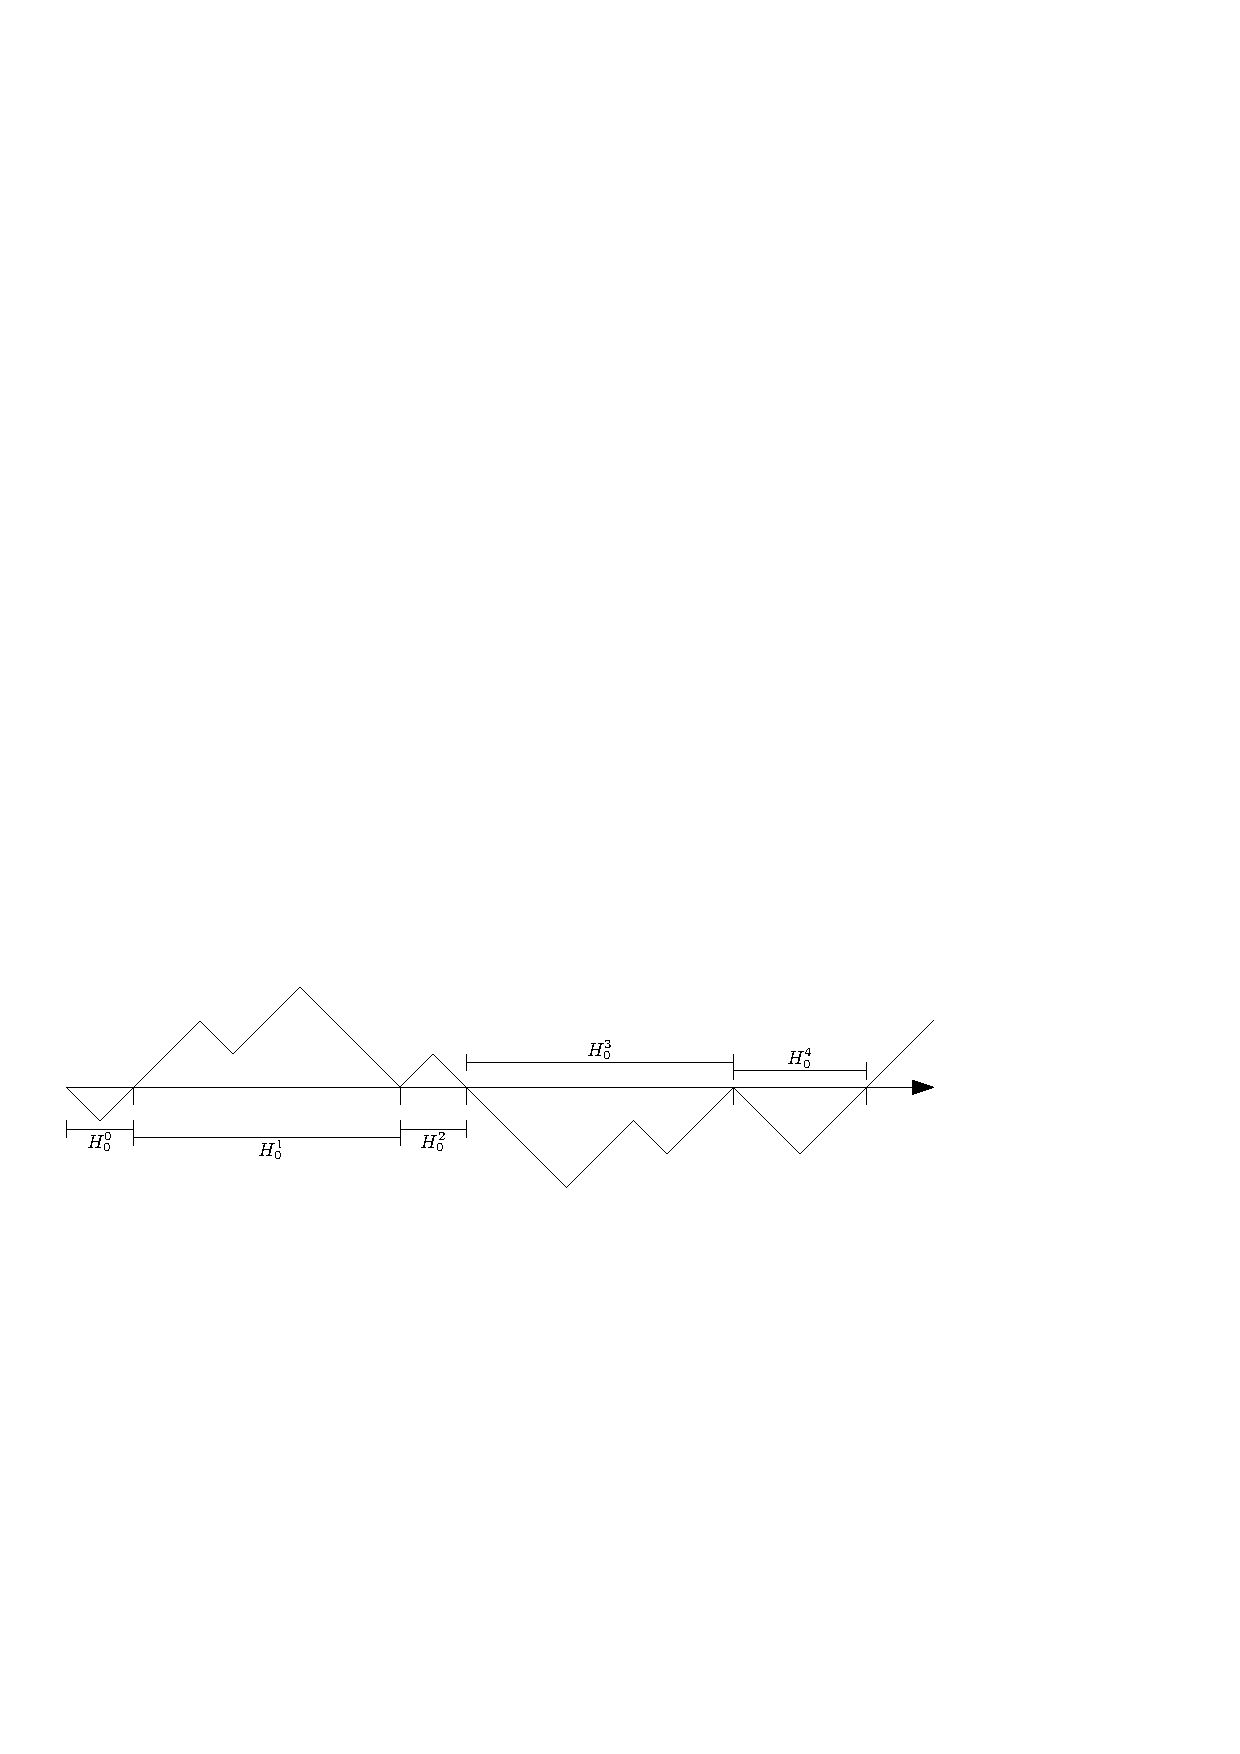
\includegraphics[width=0.8\textwidth]{figures/inter_arrival.pdf}
	\caption{Inter-arrival times for the Simple Random Walk.}
\end{figure}


\begin{lemma}[]
	Let $x,y$ with $x \leftrightarrow y$, assume $y$ is recurrent. Then for every $j \geq 1$ and $t_0, \ldots, t_j \in \mathbb{N}$:
\begin{align}
	\mathbb{P}_{x} \left[ H_y^0=t_0 \ldots H_y^j=t_j \right] = \mathbb{P}_{x} \left[ H_y=t_0 \right] \mathbb{P}_{y} \left[ H_y=t_1 \right]  \ldots  \mathbb{P}_{y} \left[ H_y=t_j \right] 
.\end{align}
Under $P_x$, $H_y^1,H_y^2, \ldots $ are i.i.d. with law $\mathbb{P}_{x} \left[ H_y^i=t \right] = \mathbb{P}_{y} \left[ H_y=t \right] $.
\end{lemma}
\begin{proof}
	Write $H^i = H_y^i$, we will prove via induction over $j$. We have $\mathbb{P}_{x} \left[ H^0 = t \right]  = \mathbb{P}_{x} \left[ H_y = y \right] $ for all $t$, showing for $j=0$.
Let $j\geq 0$ and assume that the equation holds. First note that 
	\begin{align}
	\mathbb{P}_{x} \left[ H^0 < \infty, \ldots, H^j < \infty \right] = \sum_{t_0,\ldots, t_j}^{} \mathbb{P}_{x} \left[ H^0 = t_0, \ldots, H^i=t_i \right] = \mathbb{P}_{x} \left[ H_y < \infty \right] \mathbb{P}_{y} \left[ H_y < \infty \right] ^i = 1 \\
	\color{blue} \mathbb{P}_{x} \left[ H^0 < \infty, \ldots, H^j < \infty \right] = \sum_{t_0,\ldots, t_j}^{} \mathbb{P}_{x} \left[ H^0 = t_0, \ldots, H^j=t_j \right] = \mathbb{P}_{x} \left[ H_y < \infty \right] \mathbb{P}_{y} \left[ H_y < \infty \right] ^j = 1.
	\end{align}

	Therefore $T = H^0 + \ldots + H^j$ is finite $\mathbb{P}_{x} $-a.s. and $X_T=y$. Hence, we have that for every $t_0,\ldots,t_{j+1} \in \mathbb{N}$ that
	\begin{align}
		\mathbb{P}_{x} \left[ H^0=t_0,\ldots,H^{j+1}=t_{j+1} \right] &\stackrel{\phantom{\textrm{(SMP)}}}{=} \mathbb{P}_{x} \left[ H^0 = t_0, \ldots, H^{j+1}=t_{j+1} | T<\infty, X_T = y \right]  \\
		&\stackrel{\textrm{(SMP)}}{=} \mathbb{P}_{x} \left[ H^0=t_0, \ldots, H^j=t_j \right] \mathbb{P}_{y} \left[ \min\{n> 0: X_n =y\} = t_{j+1} \right] \\ 
	&\stackrel{\phantom{\textrm{(SMP)}}}{=} \mathbb{P}_{x} \left[ X_y = t_0 \right] \mathbb{P}_{y} \left[ H_y = t_1 \right] \cdots \mathbb{P}_{y} \left[ H_y = t_{j+1} \right]  
	.\end{align}
\end{proof}

\begin{proof}[Proof (Theorem)]
	\textbf{Case 1:} $y$ transient:	we know that $\mathbb{E}_{y} \left[ V_y \right] < \infty$, thus (Strong Markov Property) $\mathbb{E}_{x} \left[ V_y \right] < \infty$. Hence for every $n> 0$,
	\begin{align}
		\frac{\mathbb{E}_{x} \left[ V_y^{(n)} \right] }{n} \leq \frac{\mathbb{E}_{x} \left[ V_x \right] }{n} \to 0
	.\end{align}
	\textbf{Case 2:} $y$ recurrent: using the lemma, we know that the random variables $H^j$ are i.i.d. under $\mathbb{P}_{x}$ and fulfill $\mathbb{E}_{x} \left[ H^1 \right] = \mathbb{E}_{y} \left[ H_y \right]  = m_y$. Then we can use the Law of Large Numbers and $\mathbb{P}_{x} \left[ H^0 < \infty \right] =1$ we find $\mathbb{P}_{x}$-a.s.,
	\begin{align}
		\lim_{i\to \infty } \frac{H^0 + \ldots + H^i}{i} = m_y
	.\end{align}
	Note that this includes the case of $m_y=\infty$ by truncation. Now we write $N_n = V_y^{(n)}$ (the number of visits to $y$ at time $n$).
	\begin{figure}[h!]
		\centering
		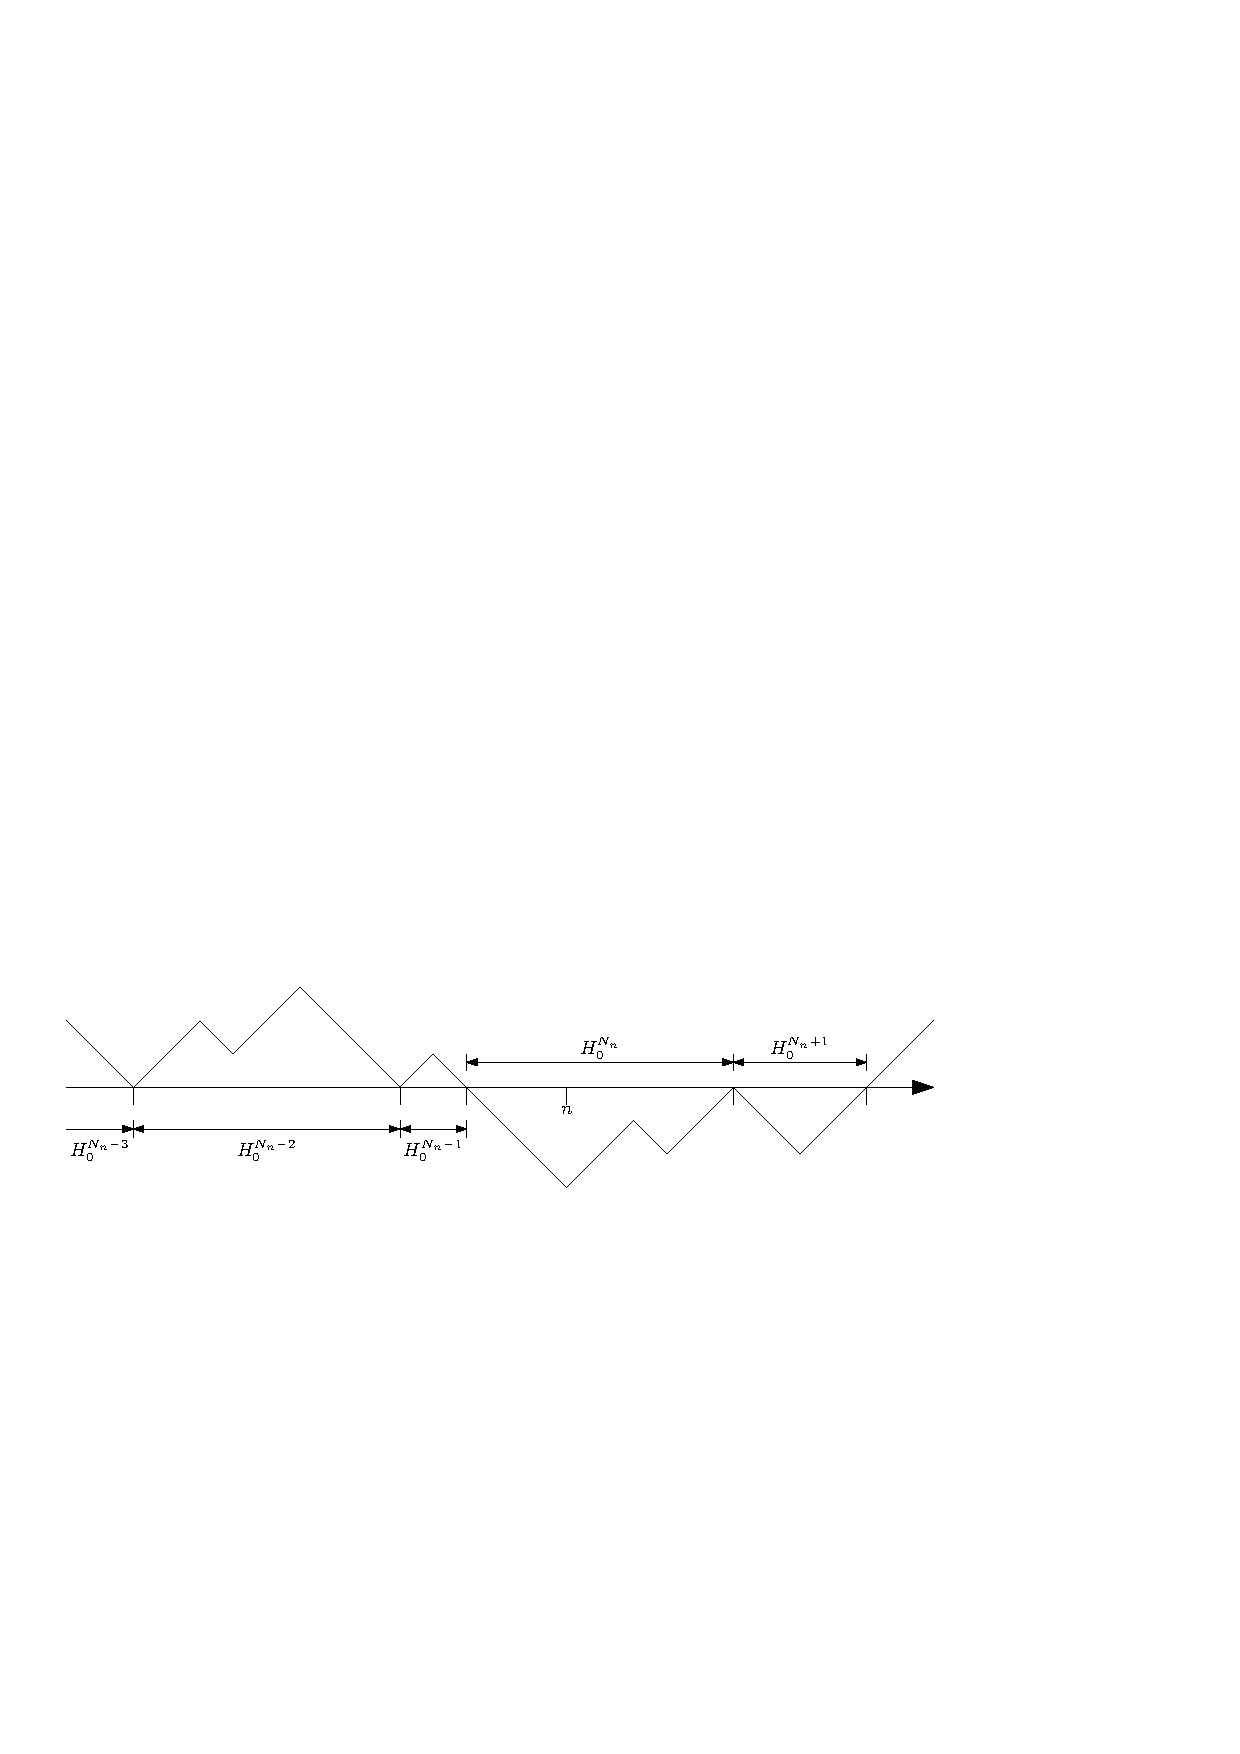
\includegraphics[width=0.8\textwidth]{figures/inter_arrival_ineq.pdf}
		\caption{Inter-arrival times of $0$ around time $n$ of the Simple Random Walk.}
	\end{figure}

Following directly from the definition of $N_n$ we have that for any $n> 0$ that 
\begin{align}
	H^0 + \ldots + H^{N_n -1} \leq n < H^0 + \ldots + H^{N_n}
.\end{align}
	
Hence, for every $n> 0$ 
\begin{align}
\frac{N_n}{H^0 + \ldots H^{N_n}} < \frac{V_y^{(n)}}{n} \leq \frac{N_n}{H^0 + \ldots + H^{N_n -1}} 
.\end{align}

The upper and lower bounds each converge to $\frac{1}{m_y}$ almost surely. Hence, we can conclude that $\mathbb{E}_{x} \left[ \frac{V_y^{(n)}}{n} \right] \to \frac{1}{m_y}$ by the Dominated Convergence Theorem.
\end{proof}


\begin{prop}[Classification of recurrent classes]
	Let $R$ be a recurrent class. Then either:
\begin{itemize}
	\item for all $x \in R,\ x$ is positive recurrent, or
	\item for all $x \in R,\ x$ is null recurrent.
\end{itemize}
\end{prop}
\begin{proof}
	Fix $x,y \in E$ with $x  \leftrightarrow  y$ and $x$ positive recurrent. Fix $k\geq 0$ with $p_{xy}^{(k)}>0$. By Chapman-Kolmogorov, we have for all $j> 0$
	\begin{align}
		p_{xy}^{(k+j)} \geq p_{xx}^{(j)} p_{xy}^{(k)}	
.	\end{align}
Thus	
\begin{align}
	\underbrace{\frac{1}{n} \sum_{i=1}^{n} p_{xy}^{(i)}}_{\to  \frac{1}{\mathbb{E}_{y} \left[ H_y \right] }} \geq \underbrace{\left( \frac{1}{n} \sum_{j=1}^{n-k} p_{xx}^{(j)} \right)}_{\to \mathbb{E}_{x} \left[ H_x \right]} \underbrace{p_{xy}^{(k)}}_{>0}
.\end{align}
Therefore, $\frac{1}{\mathbb{E}_{y} \left[ H_y \right] }> 0$ and $y$ is positive recurrent.
\end{proof}


\begin{prop}[]
	Let $R$ be a recurrent class, if $R$ is finite, then $R$ is positive recurrent. In particular, if $E$ is finite, then every recurrent state is positive recurrent.
\end{prop}
\begin{proof}
	Fix $x\in R$, since $R$ is closed we have for every $n> 0$
	\begin{align}
		1 = \mathbb{P}_{x} \left[ X_n \in R \right] = \sum_{y\in R}^{} p_{xy}^{(n)}.
	\end{align}
Hence, 
\begin{align}
	1 = \sum_{y\in R}^{} \frac{1}{n} \sum_{k=1}^{n} p_{xy}^{(k)} \to \sum_{y \in R}^{} \frac{1}{\mathbb{E}_{y} \left[ H_y \right] }.
\end{align}
Thus, there must be a $y\in R$ such that $\mathbb{E}_{y} \left[ H_y \right] < \infty $, implying that the entire class is positive recurrent.
\end{proof}


\section{Stationary Distributions for Irreducible Chains}
\begin{theorem}[]
	Assume that $p$ is irreducible. 
\begin{itemize}
	\item If the chain is transient or null recurrent, then there is no stationary distribution;
	\item if the chain is positive recurrent, then there exists a unique stationary distribution given by 
		\begin{align}
		\boxed{\pi (x) = \frac{1}{\mathbb{E}_{x} \left[ H_x \right] }}
		.\end{align}
		
\end{itemize}
\end{theorem}
\begin{proof}
	We will begin by assuming a stationary distribution $\pi$ exists. Then for every $x \in E$ we have for all $n> 0$
	\begin{align}
		\pi (x) = \frac{1}{n} \sum_{k=1}^{n} \mathbb{P}_{\pi } \left[ X_k=x \right]  = \sum_{y \in E}^{} \pi(y) \frac{1}{n} \sum_{k=1}^{n} \mathbb{P}_{y} \left[ X_k = x \right] \to \sum_{y \in E}^{} \pi (y) \frac{1}{\mathbb{E}_{x} \left[ H_x \right] }	
	.\end{align}	
	{\color{blue}Note that this also shows uniqueness of the stationary distribution.}

	Now if we assume that the chain is transient or null recurrent, then using Dominated Convergence Theorem, we have that $\pi (x) = \frac{1}{\mathbb{E}_{x} \left[ H_x \right] } = 0$. This is a contradiction to $\sum_{x \in E}^{} \pi (x) = 1$, therefore no stationary distribution can exist.

	If, instead, we assume that the chain is positive recurrent, we have the same formula as before for $\pi (x)$ as the only possible candidate for the stationary distribution. So if we can show that $\pi $ indeed defines a stationary distribution (unlike in the previous case), then we will be done. First, we fix $x> 0$ and find the inequality for all $y \in E$ 
\begin{align}
\frac{1}{\mathbb{E}_{y} \left[ H_y \right] } &\stackrel{\phantom{\textrm{(Fatou)}}}{=} \lim_{n\to \infty} \frac{1}{n} \sum_{j=k}^{n} p_{yy}^{(j)} \\
					     &\stackrel{\phantom{\textrm{(Fatou)}}}{=}  \lim_{n \to \infty} \sum_{x \in E}^{} \left( \frac{1}{n} \sum_{j=k}^{n} p_{yx}^{(j-k)} \right) p_{xy}^{(k)} \\
					     &\stackrel{\textrm{(Fatou)}}{\geq} \sum_{x \in E}^{}  \liminf_{n \to \infty } \left( \frac{1}{n} \sum_{j=k}^{n} p_{yx}^{(j-k)} \right) p_{xy}^{(k)} \\
					     &\stackrel{\phantom{\textrm{(Fatou)}}}{=}  \sum_{x \in E}^{} \frac{1}{\mathbb{E}_{x} \left[ H_x \right] } p_{xy}^{(k)}.
\end{align}
Analogously for fixed $x$
\begin{align}
	1 = \lim_{n \to \infty } \frac{1}{n} \sum_{j=1}^{n} \mathbb{P}_{x} \left[ X_j \in E \right] = \lim_{n\to \infty }\sum_{y \in E}^{}  \frac{1}{n} \sum_{j=1}^{n}\mathbb{P}_{x} \left[ X_j = y \right] \stackrel{\textrm{(Fatou)}}{\geq} \sum_{y \in E}^{} \frac{1}{\mathbb{E}_{y} \left[ H_y \right] }
.\end{align}
So we would like to prove that these two inequalities are actually inequalities. First we sum the first inequality over $y$ and get
\begin{align}
	\sum_{y \in E}^{} \frac{1}{\mathbb{E}_{y} \left[ H_y \right] } \geq \sum_{y \in E}^{} \left( \sum_{x \in E}^{} \frac{1}{\mathbb{E}_{x} \left[ H_x \right] } p_{xy}^{(k)} \right) = \sum_{x \in E}^{} \frac{1}{\mathbb{E}_{x} \left[ H_x \right] }
.\end{align}
Thus the inequality must be an equality. {\color{blue}Also note that if we can show that $\pi$ is a distribution, this also shows that it is stationary,} we have for every $k> 0$ and for all $y \in E$. 
\begin{align}
\frac{1}{\mathbb{E}_{y} \left[ H_y \right] } = \sum_{x \in E}^{} \frac{1}{\mathbb{E}_{x} \left[ H_x \right] } p_{xy}^{(k)}.	
\end{align}
We can use this to show that the second inequality is actually an equality. Fix $y \in E$ and note that $\frac{1}{\mathbb{E}_{y} \left[ H_y \right] }>0$ by positive recurrence. We have
\begin{align}
	\frac{1}{\mathbb{E}_{y} \left[ H_y \right] } &\stackrel{\phantom{\textrm{(DCT)}}}{=} \lim_{n \to \infty } \frac{1}{n} \sum_{k=1}^{n}  \left( \sum_{x \in E}^{} \frac{1}{\mathbb{E}_{x} \left[ H_x \right] } p_{xy}^{(k)} \right) \\
						     &\stackrel{\phantom{\textrm{(DCT)}}}{=} \lim_{n \to \infty }\sum_{x \in E}^{} \frac{1}{\mathbb{E}_{x} \left[ H_x \right] } \left( \frac{1}{n} \sum_{k=1}^{n} p_{xy}^{(k)} \right) \\
						     &\stackrel{\textrm{(DCT)}}{=} \sum_{x \in E}^{} \frac{1}{\mathbb{E}_{x} \left[ H_x \right] } \frac{1}{\mathbb{E}_{y} \left[ H_y \right] }
.\end{align}
Hence, $\pi(x) = \frac{1}{\mathbb{E}_{x} \left[ H_x \right] } $ defines a distribution, which is stationary.
\end{proof}


\section{Periodicity}
\begin{defn}
	Let $x \in E$. The period of $x$ is defined by
	\begin{align}
	\boxed{d_x = \gcd\{n> 0: p_{xx}^{(n)}>0\} }
	.\end{align}
	By convention $\gcd(\emptyset)=\infty$.	
\end{defn}

\begin{prop}[]
	Let $x,y$ be arbitrary elements of $ E$ then $ x \leftrightarrow y$ implies that $d_x=d_y$.
\end{prop}
\begin{proof}
	Let $x\neq y$. We prove that $d_y | d_x$. First let us fix $k,l\geq 0$ such that $p_{yx}^{(k), p_{xy}^{(l)}}> 0$. Since $p_{yy}^{(k+l)}\geq p_{yx}^{(k)}p_{xy}^{(l)}> 0$ we have that $d_y | k+l$. Now we show that $d_y$ is a common divisor of $\{n> 0: p_{xx}^{(n)}> 0\}$, this will imply our claim. For every $n> 0$ satisfying $p_{xx}^{(n)}>0$, we have 
	\begin{align}
		p_{yy}^{(k+l+n)} \geq p_{yx}^{(k)}p_{xx}^{(n)}p_{xy}^{(l)} > 0,
	\end{align}
hence $d_y | k+l+n$. Since $d_y | k+l$, we also have $d_y|n$.	
\end{proof}


\textbf{Consequence} If $p$ is irreducible we have for arbitrary $x,y \in E$ that $d_x = d_y$.

\begin{defn}
	We say that the chain $p$ is aperiodic if for every $x \in E$
	\begin{align}
	\boxed{d_x=1}.
	\end{align}
\end{defn}

\begin{prop}[]
	Let $x$ be in $E$. We have $d_x=1$ if and only if there is an $n_0 \geq 1$ such that for every $n \geq n_0$ we have that $ p_{xx}^{(n)}>0$.
\end{prop}
\begin{lemma}
	Let $A \subset \mathbb{N}\setminus \{0\}$ be stable under addition (i.e. $x,y\in A \implies x+y \in A$). Then
	\begin{align}
		\gcd (A) = 1 \iff \exists n_0 \in \mathbb{N}: \{n \in \mathbb{N}: n \geq n_0 \} \subset A.	
	\end{align}
	
\end{lemma}
\begin{proof}
	See Appendix.
\end{proof}

\begin{proof}[Proof (Proposition)]
	The set $A_x = \{n> 0: p_{xx}^{(n)}> 0\}$ under addition, because $p_{xx}^{(m+n)} \geq p_{xx}^{(m)}p_{xx}^{(n)}$ for every $m,n> 0$. The proof follows by applying the lemma to $A=A_x$.
\end{proof}


\section{Product Chain}
TODO: This needs some work with how we phrase it

\textbf{Goal} Define two Markov Chains: $X_n$ a MC$(\mu, P)$ and $\tilde{X_n}$ a MC$(\nu, P) $ on the same probability space such that $X_n = \tilde{X_n}$ for $n$ large.

\begin{figure}[h!]
	\centering
	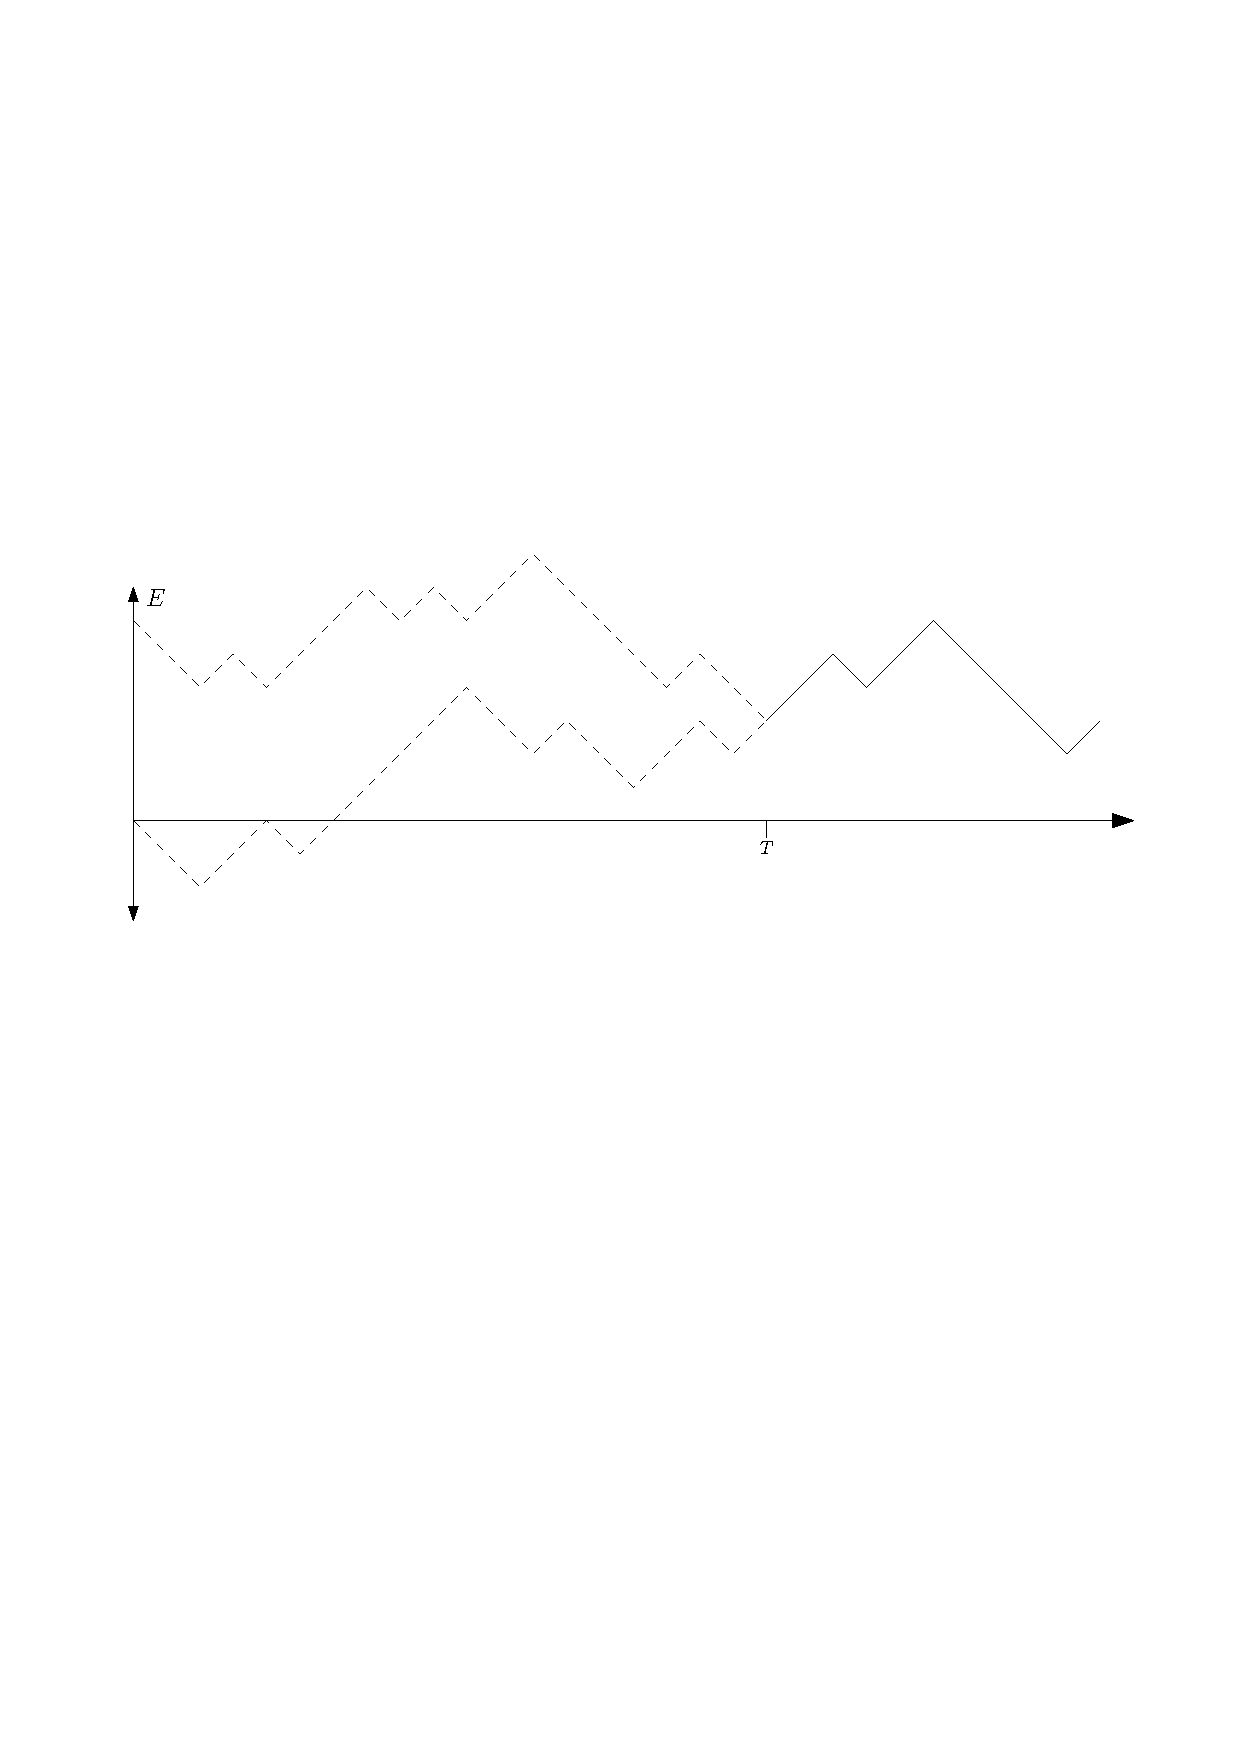
\includegraphics[width=0.8\textwidth]{figures/coupling.pdf}
	\caption{A coupling of two simple random walks started from $6$ and $0$}
\end{figure}


To achieve that we first consider two independent chains $X$ and $Y$. We then show that the chains meet almost surely (using some assumptions on $p$) at some random time $T$. Then we ask that the chains follow the same trajectory for $t>T$. In order to introduce a suitable probability space, we consider the product chain.

\begin{defn}[Product Chain]
	Define for every $\omega=(x,y), \ \omega'=(x',y') \in E^2$ 
	\begin{align}
	\boxed{\overline{p_{\omega, \omega'}}=p_{xx'}p_{yy'} }.
	\end{align}
\end{defn}
\begin{rmk}[]
	To see that $\overline{p}$ is a transition probability, calculate
	\begin{align}
		\sum_{\omega'\in E}^{} \overline{p}_{\omega \omega'} = \sum_{x',y' \in E}^{} p_{xx'}p_{yy'} = 1. 
	\end{align}
\end{rmk}


\noindent
\textbf{Notation} Consider:
\begin{itemize}
	\item $(\Omega, F, (P_\omega)_{\omega \in E^2})$ Probability Spaces,
	\item $(W_n)_{n\geq 0}=((X_n,Y_n))_{n\geq 0}$ a random variable on $(\Omega, \mathcal{F})$ such that for all $\omega \in E^2$, $W_n$ is a $MC(\delta_\omega, \overline{P})$ under $\mathbb{P}_{\omega}$.
\end{itemize}

\begin{rmk}[]
	If $\mu, \nu $ are distributions on $E$, then $\mu \otimes \nu $ is a distribution on $E^2$.
	\begin{align}
		\boxed{P_{\mu \otimes \nu }= \sum_{(x,y)\in E^2}^{}\mu (x) \nu (y) P_{(x,y)}}.
	\end{align}
	
\end{rmk}

\begin{prop}[]
	Let $\mu,\nu $ be distributions on $E$. Under $P_{\mu \otimes \nu }:$ 
\begin{itemize}
	\item $(X_n)_{n\geq 0}$ is a $MC(\mu ,P)$;
	\item $(Y_n)_{n\geq 0}$ is a $MC(\nu ,P)$.
\end{itemize}
\end{prop}
\begin{proof}
	For every $k\geq 0$ and $x_0,\ldots,x_k, y_0, \ldots, y_k \in E$ we have
\begin{align}
&	\mathbb{P}_{\mu \otimes \nu } \left[ X_0 = x_0, \ldots, X_k=x_k, Y_0 = y_0, \ldots Y_k = y_k \right] \\
&\qquad= \mathbb{P}_{\mu \otimes \nu } \left[ W_0=(x_0, y_0), \ldots, W_k = (x_k, y_k) \right] \\
&\qquad= \mu (x_0) p_{x_0x_1}\cdots p_{x_{k-1}x_k} \nu (y_0) p_{y_0 y_1} \cdots p_{y_{k-1}y_k}
.	\end{align}
Summing over all possible $y_0,\ldots , y_k$ in $E$, implies that $(X_n)_{n}$ is a MC$(\mu ,P)$, and equivalently that $(Y_n)_{n}$ is a MC$(\nu ,P)$.	

Now to show independence, we need to show that for all measurable sets $A,B \subset E^{\mathbb{N}}$ 
\begin{align}
	\mathbb{P}_{\mu \otimes \nu } \left[ X \in A, Y\in B \right] = \mathbb{P}_{\mu \otimes \nu } \left[ X \in A \right] \mathbb{P}_{\mu \otimes \nu } \left[ Y \in B \right].
\end{align}
Our calculation from before shows that this equality holds for all sets of the form $A = \{(x_0,\ldots,x_n)\} \times E^{\mathbb{N}}$, $B=E^{\mathbb{N}}\times \{(y_0,\ldots , y_n)\}$. Therefore, it holds for all cylindrical sets, and thus, by Dynkin's Lemma, for all measurable sets.
\end{proof}

\begin{prop}[]
	If $p$ is irreducible, aperiodic, and positive recurrent then $\overline{p}$ is irreducible, aperiodic, and positive recurrent.
\end{prop}


\begin{rmk}[]
	Aperiodic is important!  $p$ irreducible does not imply that $\overline{p}$ irreducible! Take $E = \{1,2\}$ and $p_{12} = p_{21}=1$, the product chain here is no longer irreducible.
\end{rmk}

\begin{figure}[h!]
\centering
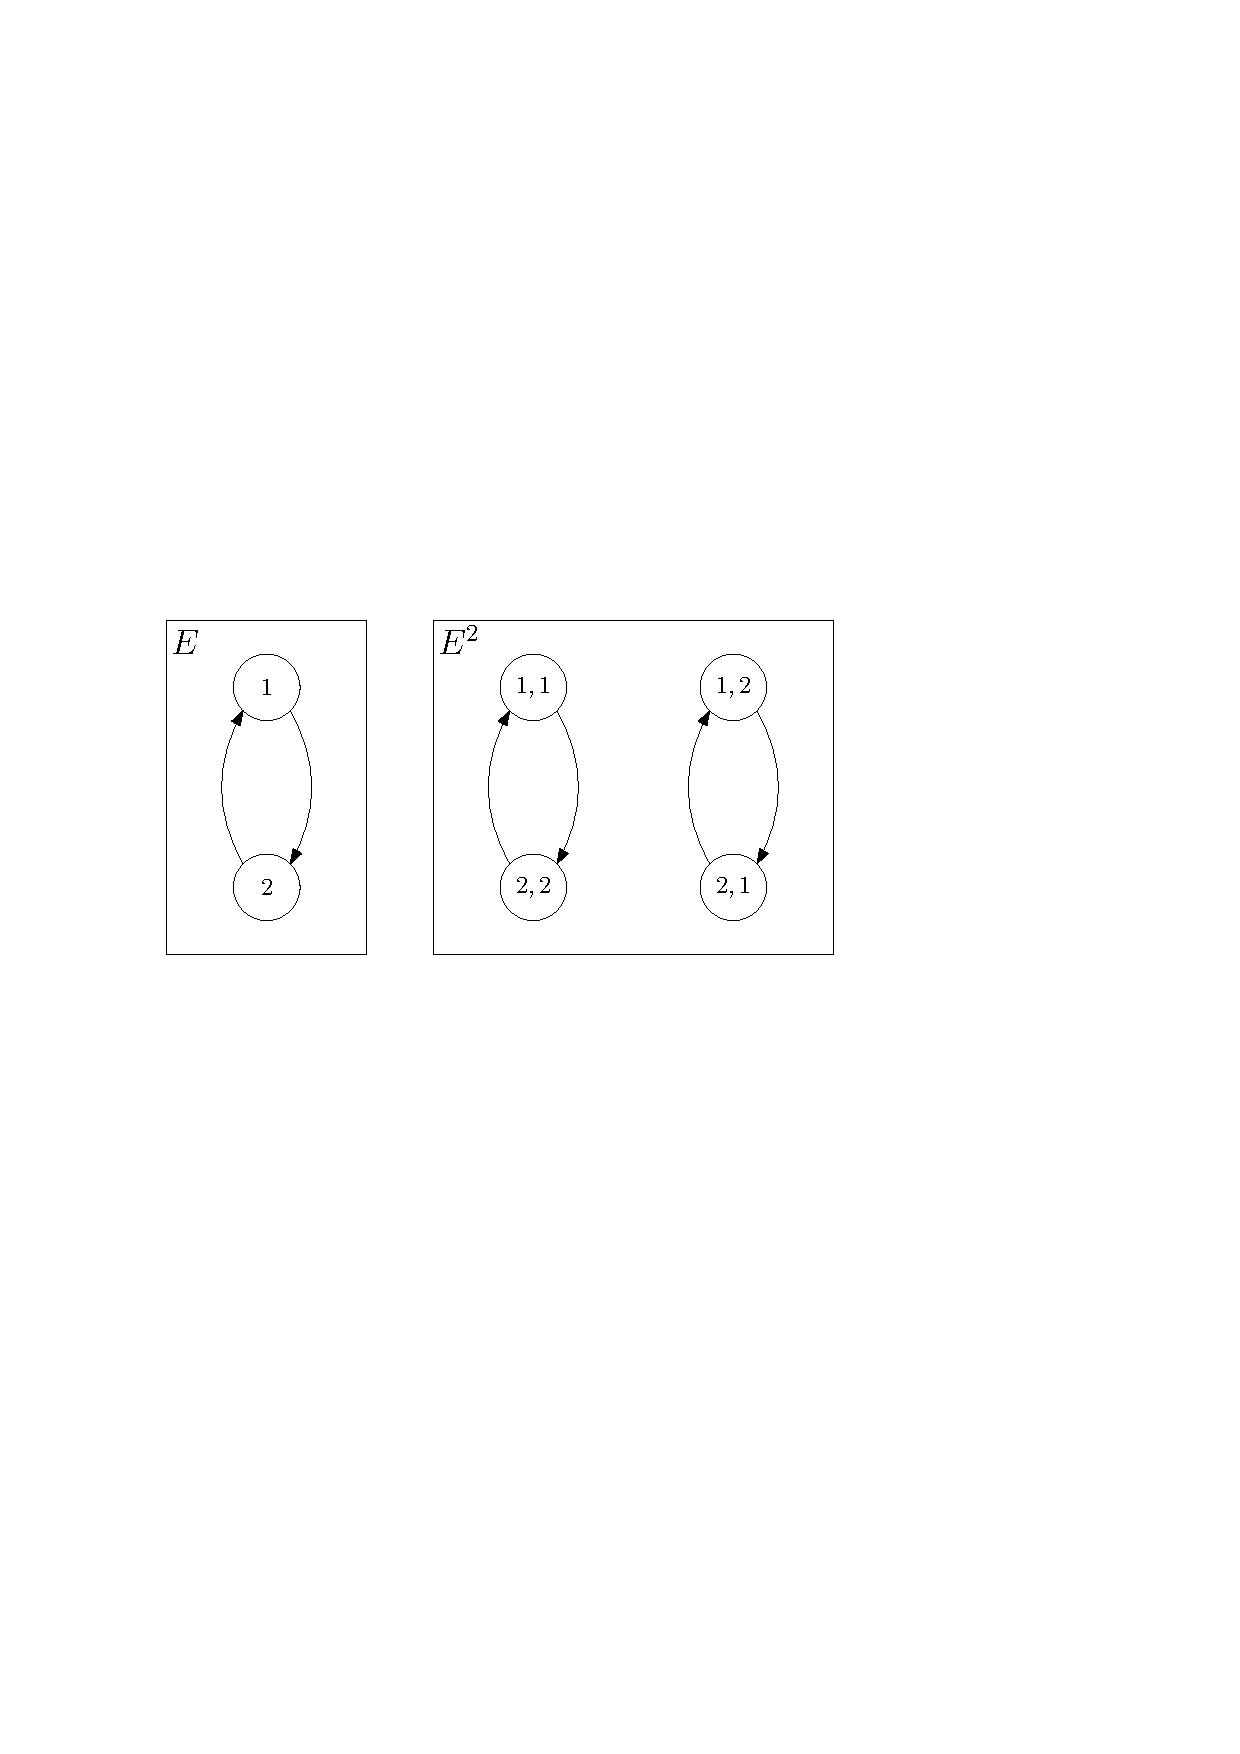
\includegraphics[width=0.6\textwidth]{figures/non_irred_prod_chain.pdf}
\caption{Example of an irreducible chain, with a reducible product chain.}
\end{figure}

\begin{proof}
	Let $w=(x,y)$ and $w'=(x',y') \in E^2$. By irreducibility we can choose $k,l\geq 0$ such that $p_{xx'}^{(k)}, p_{yy'}^{(l)} >0$. Then for every $n \gg \max(k,l)$ we have
\begin{align}
	\overline{p}_{ww'}^{(n)} = p_{xx'}^{(n)}p_{yy'}^{(n)} \geq p_{xx'}^{(k)}p_{x'x'}^{(n-k)} p_{yy'}^{(l)} p_{y'y'}^{(n-l)} > 0.
\end{align}
This holds as the two terms $p_{x'x'}^{(n-k)}$ and $p_{y'y'}^{(n-l)}$ are strictly positive for $n$ large enough.

	Since $p$ is irreducible and positive recurrent, it must admit a stationary distribution $\pi $. For every $(y,y')\in E^2$ we then have
\begin{align}
	\pi (y) \pi (y') = \sum_{x \in E}^{} \pi(x)p_{xy} \sum_{x' \in E}^{}p_{x'y'} = \sum_{(x,x')\ in E^2}^{} p_{xy}p_{x'y'}. 
\end{align}
Showing that $\pi \otimes \pi $ is stationary for $\overline{p}$, implying that $\overline{p}$ is positive recurrent.
\end{proof}

{\color{blue}
\begin{prop}[]
	If $p$ is irreducible and aperiodic, then $\overline{p}$ is irreducible and aperiodic.
\end{prop}
\begin{proof}
	Let $w=(x,y)$ and $w'=(x',y') \in E^2$. By irreducibility we can choose $k,l\geq 0$ such that $p_{xx'}^{(k)}, p_{yy'}^{(l)} >0$. Then for every $n \gg \max(k,l)$ we have
\begin{align}
	\overline{p}_{ww'}^{(n)} = p_{xx'}^{(n)}p_{yy'}^{(n)} \geq p_{xx'}^{(k)}p_{x'x'}^{(n-k)} p_{yy'}^{(l)} p_{y'y'}^{(n-l)} > 0.
\end{align}
This holds as the two terms $p_{x'x'}^{(n-k)}$ and $p_{y'y'}^{(n-l)}$ are strictly positive for $n$ large enough.
\end{proof}

\begin{prop}[]
	If $p$ is irreducible, aperiodic, and positive recurrent, then $\overline{p}$ is irreducible, aperiodic, and positive recurrent.
\end{prop}
\begin{proof}
	We only have to show that the product chain is positive recurrent, as the other properties follow from the previous proposition. Since $p$ is irreducible and positive recurrent, it must admit a stationary distribution $\pi $. For every $(y,y')\in E^2$ we then have
\begin{align}
	\pi (y) \pi (y') = \sum_{x \in E}^{} \pi(x)p_{xy} \sum_{x' \in E}^{}p_{x'y'} = \sum_{(x,x')\ in E^2}^{} p_{xy}p_{x'y'}. 
\end{align}
Showing that $\pi \otimes \pi $ is stationary for $\overline{p}$, implying that $\overline{p}$ is positive recurrent.
\end{proof}
}
\begin{defn}
	$T=\min\{n\geq 0: X_n=Y_n\}$ is a stopping time.
\end{defn}
\begin{rmk}[]
	In fact for $A = \{ (x,y) \in E^2: x=y\}$ (which is measurable) $T=H_A$, so $T$ is a stopping time.
\end{rmk}


\begin{prop}[]
	For $\mu, \nu $ distributions on $E$, $n\geq 0$: 
\begin{align}
	\boxed{ \sum_{x \in E}^{} |\mathbb{P}_{\mu } \left[ X_n=x \right] - \mathbb{P}_{\nu} \left[Y_n=x  \right] | \leq 2 \mathbb{P}_{\mu \otimes \nu } \left[ T>n \right] }
.\end{align}
\end{prop}
\begin{proof}
	We consider the product Markov Chain $W_n = (X_n, Y_n)$ under $\mathbb{P}_{\mu \otimes \nu}$. We then define, for every $n$ 
	\begin{align}
		\tilde{X}_n =
	\begin{cases}
		Y_n & \textrm{for } n < T \\
		X_n & \textrm{for } n \geq T
	\end{cases}
	.\end{align}

We now show that $(\tilde{X}_n)$ is a MC$(\nu, P)$ under $\mathbb{P} = \mathbb{P}_{\mu \otimes \nu}$. Let $n\geq 0$ and $x_0, \ldots, x_n \in E$. Now we distinguish between possible values for $T$ and find
\begin{align}
	\mathbb{P}_{} \left[ \tilde{X}_0 = x_0, \ldots , \tilde{X}_n = x_n \right] = \sum_{k \in \mathbb{N} \cup \{\infty\}}^{} \mathbb{P}_{} \left[ \tilde{X}_0 = x_0, \ldots , \tilde{X}_n , T=k \right] .
\end{align}
If $k>n$, the summand is equal to 
\begin{align}
	\nu (x_0) p_{x_0x_1}\cdots p_{x_{n-1}x_n} \cdot \mathbb{P}_{} \left[ T=k | Y_0 = x_0, \ldots , Y_n=x_n \right].
\end{align}
If $k \leq n$, the summand is equal to
\begin{align}
	&\mathbb{P}_{} \left[ \underbrace{Y_0=x_0, \ldots , Y_k=x_k,T=k}_{\in \mathcal{F}_T},X_{T+1}=x_{k+1}, \ldots X_{T+n-k}=x_n \right]  \\
	&\qquad \stackrel{\textrm{(SMP)}}{=} \mathbb{P}_{} \left[ Y_0=x_0, \ldots Y_k=x_k, T=k \right] \mathbb{P}_{(x_k, x_k)} \left[ X_1=x_{k+1}, \ldots , X_{n-k}=x_n \right]  \\
	&\qquad \stackrel{\phantom{\textrm{(SMP)}}}{=} \nu (x_0) p_{x_0x_1}\cdots p_{x_{k-1}x_k} \mathbb{P}_{} \left[ T=k | Y_0 = y_0, \ldots, Y_k=x_k \right] p_{x_k x_{k+1}} \cdots p_{x_{n-1}x_n}  \\
	&\qquad \stackrel{\phantom{\textrm{(SMP)}}}{=} \nu (x_0) p_{x_0 x_1} \cdots p_{x_{n-1}x_n} \mathbb{P}_{} \left[ T=k | Y_0=x_0, \ldots, Y_n=x_n \right]  .
\end{align}
To justify the last equality, we used the independence between $(X_n)$ and $(Y_n)$ to write
 \begin{align}
	 \mathbb{P}_{} \left[ T=k | Y_0=x_0, \ldots , Y_k =x_k \right] &= \mathbb{P}_{} \left[ \forall i<k\ X_i \neq x_i, X_k=x_k \right] \\
								       &= \mathbb{P}_{} \left[ T=k | Y_0=x_0, \ldots , Y_n=x_n \right] . 
\end{align}
Finally using that $\sum_{k \in \mathbb{N}\cup \{\infty\}}^{} \mathbb{P}_{} \left[ T=k | Y_0 = x_0, \ldots , Y_n =x_n \right] =1$ we obtain
\begin{align}
	\mathbb{P}_{} \left[ \tilde{X}_0 = x_0, \ldots , \tilde{X}_n=x_n \right] = \nu (x_0) p_{x_0 x_1} \cdots p_{x_{n-1}x_n}.
\end{align}

Using the coupling between $X$ and $\tilde{X}$ to conclude that for every $n\geq 0$ 
\begin{align}
	\sum_{x \in E}^{} \left| \mathbb{P}_{\mu} \left[ X_n = x \right] - \mathbb{P}_{\nu } \left[ X_n=x \right] \right|
	&= \sum_{x \in E}^{} \left| \mathbb{P}_{} \left[X_n =x  \right] - \mathbb{P}_{} \left[ \tilde{X}_n = x \right] \right| \\
	&= \sum_{x \in E}^{} \Big| \mathbb{P}_{} \left[ X_n =x, T \leq n \right] + \mathbb{P}_{} \left[ X_n = x, T>n \right] \\
	&\qquad  - \mathbb{P}_{} \left[ \tilde{X}_n = x, T \leq n \right] + \mathbb{P}_{} \left[ \tilde{X}_n = x, T>n \right] \Big| \\
	&\leq \sum_{x \in E}^{} \mathbb{P}_{} \left[ X_n=x, T>n \right] + \mathbb{P}_{} \left[ \tilde{X}_n=x, T>n \right]\\
	&= 2\mathbb{P}_{} \left[ T>n \right] 
\end{align}
\end{proof}

{\color{blue} // I would separate the proof into a lemma and then proof of the proposition//
\begin{lemma}[]
	$\tilde{X}_n = Y_n \mathbbm{1}_{\{T<n\}} + X_n \mathbbm{1}_{\{T \geq n\}} $ is a $MC(\nu, P)$.
\end{lemma}
\begin{proof}
	We consider the product Markov Chain $W_n = (X_n, Y_n)$ under $\mathbb{P}_{\mu \otimes \nu}$. We then define, for every $n$ 
	\begin{align}
		\tilde{X}_n =
	\begin{cases}
		Y_n & \textrm{for } n < T \\
		X_n & \textrm{for } n \geq T
	\end{cases}
	.\end{align}

We now show that $(\tilde{X}_n)$ is a MC$(\nu, P)$ under $\mathbb{P} = \mathbb{P}_{\mu \otimes \nu}$. Let $n\geq 0$ and $x_0, \ldots, x_n \in E$. Now we distinguish between possible values for $T$ and find
\begin{align}
	\mathbb{P}_{} \left[ \tilde{X}_0 = x_0, \ldots , \tilde{X}_n = x_n \right] = \sum_{k \in \mathbb{N} \cup \{\infty\}}^{} \mathbb{P}_{} \left[ \tilde{X}_0 = x_0, \ldots , \tilde{X}_n , T=k \right] .
\end{align}
If $k>n$, the summand is equal to 
\begin{align}
	\nu (x_0) p_{x_0x_1}\cdots p_{x_{n-1}x_n} \cdot \mathbb{P}_{} \left[ T=k | Y_0 = x_0, \ldots , Y_n=x_n \right].
\end{align}
If $k \leq n$, the summand is equal to
\begin{align}
	&\mathbb{P}_{} \left[ \underbrace{Y_0=x_0, \ldots , Y_k=x_k,T=k}_{\in \mathcal{F}_T},X_{T+1}=x_{k+1}, \ldots X_{T+n-k}=x_n \right]  \\
	&\qquad \stackrel{\textrm{(SMP)}}{=} \mathbb{P}_{} \left[ Y_0=x_0, \ldots Y_k=x_k, T=k \right] \mathbb{P}_{(x_k, x_k)} \left[ X_1=x_{k+1}, \ldots , X_{n-k}=x_n \right]  \\
	&\qquad \stackrel{\phantom{\textrm{(SMP)}}}{=} \nu (x_0) p_{x_0x_1}\cdots p_{x_{k-1}x_k} \mathbb{P}_{} \left[ T=k | Y_0 = y_0, \ldots, Y_k=x_k \right] p_{x_k x_{k+1}} \cdots p_{x_{n-1}x_n}  \\
	&\qquad \stackrel{\phantom{\textrm{(SMP)}}}{=} \nu (x_0) p_{x_0 x_1} \cdots p_{x_{n-1}x_n} \mathbb{P}_{} \left[ T=k | Y_0=x_0, \ldots, Y_n=x_n \right]  .
\end{align}
To justify the last equality, we used the independence between $(X_n)$ and $(Y_n)$ to write
 \begin{align}
	 \mathbb{P}_{} \left[ T=k | Y_0=x_0, \ldots , Y_k =x_k \right] &= \mathbb{P}_{} \left[ \forall i<k\ X_i \neq x_i, X_k=x_k \right] \\
								       &= \mathbb{P}_{} \left[ T=k | Y_0=x_0, \ldots , Y_n=x_n \right] . 
\end{align}
Finally using that $\sum_{k \in \mathbb{N}\cup \{\infty\}}^{} \mathbb{P}_{} \left[ T=k | Y_0 = x_0, \ldots , Y_n =x_n \right] =1$ we obtain
\begin{align}
	\mathbb{P}_{} \left[ \tilde{X}_0 = x_0, \ldots , \tilde{X}_n=x_n \right] = \nu (x_0) p_{x_0 x_1} \cdots p_{x_{n-1}x_n}.
\end{align}
\end{proof}
\begin{proof}[Proof (Proposition)]
We can now take advantage of the coupling between $X$ and $\tilde{X}$ to conclude that for every $n\geq 0$ 
\begin{align}
	\sum_{x \in E}^{} \left| \mathbb{P}_{\mu} \left[ X_n = x \right] - \mathbb{P}_{\nu } \left[ X_n=x \right] \right|
	&= \sum_{x \in E}^{} \left| \mathbb{P}_{} \left[X_n =x  \right] - \mathbb{P}_{} \left[ \tilde{X}_n = x \right] \right| \\
	&= \sum_{x \in E}^{} \Big| \mathbb{P}_{} \left[ X_n =x, T \leq n \right] + \mathbb{P}_{} \left[ X_n = x, T>n \right] \\
	&\qquad  - \mathbb{P}_{} \left[ \tilde{X}_n = x, T \leq n \right] + \mathbb{P}_{} \left[ \tilde{X}_n = x, T>n \right] \Big| \\
	&\leq \sum_{x \in E}^{} \mathbb{P}_{} \left[ X_n=x, T>n \right] + \mathbb{P}_{} \left[ \tilde{X}_n=x, T>n \right]\\
	&= 2\mathbb{P}_{} \left[ T>n \right] 
\end{align}
\end{proof}
}


\section{Convergence for Irreducible Aperiodic Chains}
\begin{theorem}[]
	Assume $p$ is irreducible and aperiodic, and admits a stationary distribution $\pi $. Then for every distribution $\mu$ on $E$ and $x \in E$  
	\begin{align}
\boxed{	\lim_{n \to \infty}\mathbb{P}_{\mu } \left[ X_n=x \right] = \pi(x)}
	.\end{align}
	

	\noindent
	Equivalently: Under $\mathbb{P}_\mu: $ $X_n \stackrel{(law)}{\to} X_\infty$ where $X_\infty \sim \pi$. 

	\noindent
	Equivalently: For all $f:E\to \mathbb{R}$ bounded: $\lim_{n \to \infty} \mathbb{E}_{\mu } \left[ f(X_n) \right] = \int_{E}^{} f d \pi$.
\end{theorem}
\begin{proof}
	Consider the product chain $(X_n, Y_n)_{n\geq 0}$ as before. We know that $\overline{P}$ is irreducible and positive recurrent, furthermore the stopping time $T=\min\{n\geq 0: X_n = Y_n\}$ is $\mathbb{P}_{\mu \otimes \pi }$-a.s. finite. To check this last claim, simply note that $T \leq H_{(a,a)}$ for any $a$ fixed. Then we have that for every $x \in E$ 
\begin{align}
	\left| \mathbb{P}_{\mu } \left[ X_n = x \right] - \pi(x) \right| = \left|\mathbb{P}_{\mu } \left[ X_n = x \right] - \mathbb{P}_{\pi } \left[ X_n = x \right] \right| \leq 2 \mathbb{P}_{\mu \otimes \pi } \left[ T >n \right] \to 0 
	.\end{align}
\end{proof}


\begin{theorem}[]
	Assume that $P$ is irreducible, aperiodic, and null recurrent or transient. Then for every distribution $\mu $ and every $x \in E$  
	\begin{align}
\boxed{	\lim_{n \to \infty}\mathbb{P}_{\mu } \left[ X_n =x \right] = 0 }
.	\end{align}
	
\end{theorem}
\begin{lemma}[]
	$\overline{P}$ irreducible and recurrent, then for every $\mu $ distribution on $E$, any $i\geq 0$, and every $x \in E$
	\begin{align}
	\lim_{n \to \infty} | \mathbb{P}_{\mu } \left[ X_n=x \right] - \mathbb{P}_{\mu } \left[ X_{n+i}=x \right] | = 0
	\end{align}
\end{lemma}
\begin{proof}
	Define the distribution $\mu_i(y) = \mathbb{P}_{\mu } \left[ X_i = y \right] $, {\color{blue}'the $i$-step initial distribution'} '$\mu_i=\mu P^i$'. Next, observe that
\begin{align}
	\mathbb{P}_{\mu _i} \left[ X_n = x \right] &= \sum_{y \in E}^{} \mu _i \mathbb{P}_{y} \left[ X_n = x \right] 
	\stackrel{\textrm{(SiMP)}}{=} \sum_{y \in E}^{} \mathbb{P}_{\mu } \left[ X_i = y \right] \mathbb{P}_{\mu } \left[ X_{n+i} | X_i = y\right] 
	= \mathbb{P}_{\mu } \left[ X_{n+i}=x \right] 
\end{align}

Now, if we consider the product chain $(X_n, Y_n)_{n\geq 0}$ under $\mathbb{P}_{\mu \otimes \mu_i} $ and define the stopping time $T= \min\{n\geq 0: X_n = Y_n\}$. Here, we have that $T<\infty$ almost surely as $\overline{P}$ is recurrent. Hence we find that
\begin{align}
	\left| \mathbb{P}_{\mu } \left[ X_n = x \right] - \mathbb{P}_{\mu } \left[ X_{n+i} = x \right] \right|
	= \left| \mathbb{P}_{\mu } \left[ X_n = x \right] - \mathbb{P}_{\mu} \left[ X_n = x \right] \right| 
	\leq 2  \mathbb{P}_{\mu \otimes \mu _i} \left[ T>n \right]  \to 0.
\end{align}
\end{proof}
\begin{proof}[Proof (Theorem)]
	\textbf{Case 1:} 
	Assume $\overline{P}$ transient. Consider the product chain $(X_n, Y_n)$ under $\mathbb{P}_{\mu \otimes \mu }$, since $(x,x)$ is a transient state the last visit time $L=\max\{n\geq 0: (X_n, Y_n)=(x,x)\}$ is finite $\mathbb{P}_{\mu \otimes \mu}$-a.s. Hence,

	{\color{blue}
	Assume $\overline{P}$ transient. If we look at the product chain $(X_n, Y_n)$ under $\mathbb{P}_{\mu \otimes \mu}$, we can see that $(x,x)$ is a transient state. Thus the time of the last visit  $L = \max\{n\geq 0: (X_n, Y_n) = (x,x) \}$ is finite $\mathbb{P}_{\mu \otimes \mu}$-a.s. (if this was not almost sure, then we would have a non-zero probability that $(x,x)$ is revisited infinitely often, thus by the Dichotomy Theorem $(x,x)$ would be recurrent). Hence, 
}
\begin{align}
	\mathbb{P}_{\mu } \left[ X_n = x \right]^2 = \mathbb{P}_{\mu \otimes \mu} \left[ X_n =x, Y_n=x \right] \leq \mathbb{P}_{\mu \otimes \mu } \left[ L \geq n \right] \to 0.
\end{align}

\textbf{Case 2:} Assume $\overline{P}$ is null recurrent, fix  $y \in E$. We would like to prove that $p_{yx}^{(n)} \to 0$. To do this fix $\epsilon > 0$ and choose $k$ such that
\begin{align}
	\frac{1}{k+1} \sum_{i\leq k}^{} p_{xx}^{(i)} < \epsilon.
\end{align}
{\color{blue}We can choose such a $k$ using the density of visits theorem and that $(x,x)$ is null recurrent.} Now define the stopping time $H = \min\{j \geq n: X_j = x\}${\color{blue}, 'the first hit time of $x$ after time $n$'}. So for every $n\geq 0$ we have
\begin{align}
	\frac{1}{k+1} \sum_{i=0}^{k} \mathbb{P}_{\mu } \left[ X_{n+1}=x \right]  \leq \frac{1}{k+1} \sum_{i=0}^{k} \mathbb{P}_{\mu } \left[ X_{H+i}=x \right]  
	\stackrel{\textrm{(SMP)}}{=} \frac{1}{k+1} \sum_{i=0}^{k} \mathbb{P}_{x} \left[ X_i =x \right]  \leq \epsilon.
\end{align}
{\color{blue}The first inequality can be justified by noticing that the probability of the chain hitting $x$ after $n$ and before $ H$ is 0.} Hence,
\begin{align}
	\mathbb{P}_{\mu } \left[ X_n = x \right] &= \frac{1}{k+1} \sum_{i=0}^{k} \mathbb{P}_{\mu } \left[ X_n = x \right] \\
						 &\leq \underbrace{\frac{1}{k+1}\sum_{i=0}^{k} \left| \mathbb{P}_{\mu } \left[ X_n = x \right] - \mathbb{P}_{\mu } \left[ X_{n+i} = x \right] \right|}_{\to 0} + \underbrace{\frac{1}{k+1} \sum_{i=0}^{k} \mathbb{P}_{\mu } \left[ X_{n+i}=x \right]}_{\leq \epsilon} 
.\end{align}
Using the lemma ($\overline{P}$ is irreducible and recurrent) we find that
\begin{align}
	\limsup_{n\to\infty} \mathbb{P}_{\mu } \left[ X_n = x \right] \leq \epsilon.
\end{align}
\end{proof}

{\color{blue}\textbf{Applications} 
	In practice we may not be able to identify the stationary distribution analytically, in which case we can instead simulate the chain and record its path. The empirical distribution this process yields will then converge towards the stationary distribution. 

	Alternatively, we may want to generate samples from a given distribution, under certain conditions a direct approach using the cumulative distribution function may prove ineffective. Thus we can instead create a Markov Chain with stationary distribution as our desired distribution (by choosing the transition probabilities correctly), simulating this chain will then give us samples (in the limit) which are distributed like our target distribution.
}

\noindent \textbf{Conclusion} We previously asked the following questions:
\begin{itemize}
	\item If we fix $x \in E$, will the chain visit $x$ infinitely many times?
	\item What is the behavior of $X_n$ for $n$ large?
\end{itemize}
Now we are equipped to answer them using our ideas of recurrence/transience and the theorem for existence (and uniqueness) of stationary distributions for an irreducible chain. We were also found that using coupling we find that if we let the chain evolve for a long time, then the distribution of $X_n$ actually converges to the stationary distribution (where this distribution is 0 everywhere if a stationary distribution does not exist).


